\documentclass[11pt]{article}

%%%%%%%%%%%%%%%%%%%%%%%%%%%%%% Package Imports %%%%%%%%%%%%%%%%%%%%%%%%%%%%%%
\usepackage[normalem]{ulem}
\usepackage[utf8]{inputenc}
\usepackage[T1]{fontenc}
\usepackage{graphicx}
\usepackage[colorinlistoftodos]{todonotes}
\usepackage[english]{babel}
\usepackage{silence}
\WarningFilter{hyperref}{Token not allowed in a PDF string} % Suppress hyperref warnings about special characters in PDF bookmarks and headers
\usepackage[colorlinks=true, allcolors=titleblue]{hyperref}
\addto\extrasenglish{%
  \renewcommand{\sectionautorefname}{Section}%
  \renewcommand{\subsectionautorefname}{Subsection}%
  \renewcommand{\subsubsectionautorefname}{Subsubsection}%
}

\usepackage{setspace}

\usepackage[font=normalsize, justification=raggedright, singlelinecheck=false, textfont=bf, labelfont=bf]{caption}
\usepackage{subcaption}
\usepackage{xcolor}
\usepackage{float}
\usepackage{titling} 
\usepackage{blindtext}
\usepackage{siunitx}
\usepackage[square,sort,comma,numbers]{natbib}
\usepackage{tikz}
\usepackage{geometry}
\usepackage{amsmath}
\usepackage{tikzpagenodes}
\usepackage{tabularx}
\usepackage{tabularray}
\usepackage{booktabs}
\usepackage{listings}
\usepackage{nicefrac}
\usepackage{bm}
\definecolor{dunkelorange}{RGB}{204, 102, 0}
\definecolor{darkgreen}{rgb}{0.0, 0.4, 0.0}
\definecolor{codegreen}{rgb}{0,0.5,0.1}
\definecolor{codegray}{rgb}{0.5,0.5,0.5}
\definecolor{codepurple}{rgb}{0.58,0,0.67}
\definecolor{backcolour}{rgb}{0.92,0.94,0.96}
\definecolor{keywordcolor}{rgb}{0.8, 0.2, 0.4}
\definecolor{titleblue}{rgb}{0.2, 0.4, 0.6}

\lstdefinestyle{mystyle}{
    backgroundcolor=\color{backcolour},   
    commentstyle=\color{codegreen},
    keywordstyle=\color{keywordcolor},
    numberstyle=\tiny\color{codegray},
    stringstyle=\color{codepurple},
    basicstyle=\ttfamily\footnotesize,
    breakatwhitespace=false,         
    breaklines=true,                 
    captionpos=b,                    
    keepspaces=true,                 
    numbers=left,                    
    numbersep=5pt,                  
    showspaces=false,                
    showstringspaces=false,
    showtabs=false,                  
    tabsize=2
}
\lstset{style=mystyle}
\definecolor{tudelftdarkblue}{RGB}{12,35,64}
\definecolor{tudelftcyan}{RGB}{0,166,214}
\definecolor{tudelftblue}{RGB}{0, 118, 194}
\geometry{a4paper, margin=2cm}

% Space
\setlength{\abovedisplayskip}{1.5cm}
\setlength{\belowdisplayskip}{1.5cm}
\setlength{\abovedisplayshortskip}{0.9cm}
\setlength{\belowdisplayshortskip}{0.9cm}

\usepackage{helvet}
\renewcommand{\familydefault}{\sfdefault}
\setlength\parindent{0pt} %set no indent
\numberwithin{table}{section}
\numberwithin{figure}{section}
\newcolumntype{K}[1]{>{\centering\arraybackslash}p{#1}}
\newcolumntype{C}{>{\centering\arraybackslash}X}

\newcommand{\imgscale}{0.7}

\usepackage{titlesec}
% Kapitel ohne Nummern
\titleformat{\chapter}[display]
  {\normalfont\Huge\bfseries} % Schriftart und Stil
  {} % Kapitelnummer weglassen
  {0pt} % Abstand zwischen Nummer (hier keine) und Titel
  {} % Titel selbst
%%%%%%%%%%%%%%%%%%%%%%%%%%%%%%%%%%%%%%%%%%%%%%%%%%%%%%%%%
\usepackage{array}
\newcolumntype{P}[1]{>{\centering\arraybackslash}p{#1}}

\begin{document}

\setstretch{1.2}

% !TeX root = ../main.tex
\begin{titlepage}
    \fontfamily{RobotoSlab-TLF}\selectfont 
    \vspace*{3cm}
    
    \centering
    {\Huge \textbf{\textcolor{black}{Main Title\\[0.6cm] \LARGE Sub Title}}}\\[1.5cm]
    \textsc{\LARGE Course}\\[0.5cm]
    \text{\large Coursenumber}\\[2cm]
    
    {\Large \textbf{\textcolor{tudelftdarkblue}{Author:}}}\\[0.5cm]
    \begin{tabular}{c}        
        \Large \textcolor{tudelftdarkblue}{Felix Vossbrink (6547834)} \\
        \Large \textcolor{tudelftdarkblue}{Nikolay Ganozliev (5463912)} \\
        \Large \textcolor{tudelftdarkblue}{Sten Smilde (5375274)} \\
    \end{tabular}\\[2cm]
    
    {\Large \textcolor{tudelftdarkblue}{\today}}
    
    \vfill
    \begin{center}
        
\includegraphics[width=0.6\textwidth]{plots/logo}
    \end{center}
\end{titlepage}

%%% Create a table of contents
\tableofcontents
\newpage

%%%Insert all the chapters
\section{Introduction}
\subsection{Expectations}
At the beginning of this project, we explored several concepts for an electric vehicle, aiming to go beyond the standard passenger car. We initially considered a performance-oriented Formula E platform as well as a high-efficiency commuting car. However, since individual commuting is fundamentally inefficient as a concept, we looked for more impactful solutions. Rail transport, for instance, is significantly more efficient per ton-kilometer. This led us to combine our interests in performance and efficiency by investigating the electrification of heavy-haul freight trains.

Specifically, the famous Mauritanian Iron Ore Train, which transports ore from inland mines to the coast. This project is particularly compelling because of the theoretical abundance of solar energy in the region. However, the Sahara’s harsh desert environment presents a major engineering challenge for electrification. Currently, the train relies on diesel-electric locomotives operating in a series-hybrid configuration \cite{SNIM2024NIES}. In 2023, the emissions from this operation exceeded 75,000 tons of CO2 equivalents (CO2e), which is roughly equal to the annual carbon footprint of 7,500 average EU households \cite{SNIM2023AnnualReport, Ivanova2017Mapping}.

 After having the idea, further research also showed that we are not the first to explore this potential. During the 2023 United Nations Climate Change Conference (COP28), a memorandum was signed to explore electrifying the rail corridor using green hydrogen \cite{SNIM2023AnnualReport}, which lead us to the conclusion that there is a real use case for this project.

In contrast to most vehicle design projects, presented in the course, this project aims to design a vehicle for one specific usecase on one specific track. Although it can function as a role model for the electrification of heavy duty trains in remote and arid regions, its parameters are designed and optimized for its specific track, mass and usecase. The expectation was therefore not to create a vehicle that could be used and tested in different driving cycles, but to create an electrified version of the train and the necessary infrastructure, specifically designed for the driving cycle of transporting the iron ore from the mines to the sea, and the empty train back. Thus the design process started, by looking at the current trains specifications and its track. 

\subsection{Vehicle Specifications}
In~\autoref{tab:vehicle_specs}, key numbers for the currently operating train are summarized. It has to be noted that during the research only little information about quantitative vehicle specifications could be found, which left room for some interpretation and educated guesses, e.g. by comparing other heavy duty trains.  

\begin{table}[ht]
    \centering
    \caption{Vehicle specifications of the iron ore train \cite{SNIM2024NIES}.}
    \label{tab:vehicle_specs}
    \begin{tblr}{
        colspec={l X},
        column{1} = {font=\bfseries},
        hlines,
        vlines,
    }
        Purpose & Transport of Iron Ore \\
        Length & 2500 m \\
        Weight & 5000 t (empty) - 22000 t (loaded) \\
        Top Speed &  65 km/h (empty) - 45 km/h (loaded) \\
        Max. Gradient & 0.36\% \\
        Acceleration & below 0.1 m/s\textsuperscript{2} \\
        Track Length & 700 km
    \end{tblr}
\end{table}

The current train is operated in several configurations, typically consisting of four diesel locomotives pulling between 200 and 220 ore wagons, along with two additional carriages for mining staff. The power requirements for the operation can be divided into two distinct segments. On the outbound journey to the mines, the train is empty but must overcome a steady positive gradient, as the mines sit at an elevation of approximately 390 m above sea level \cite{ASECNA2024}.

On the return journey to the port, the situation is reversed. Although the train is significantly heavier due to the ore load, much of the route follows a negative gradient, which reduces the net energy required for propulsion. However, the "main crux" of the entire track is a relatively steep uphill section located shortly after leaving the mines toward the port \autoref{fig:track_profile}. This specific segment is a critical design parameter, as it determines the steady-state peak power the locomotives must provide to move the fully loaded mass. Using google earth elevation data~\cite{googleearth2026}, a gradient map of the track was extracted. This profile served as the basis for determining the train's specific driving cycle in the following sections.

\begin{figure}[ht]
    \centering
    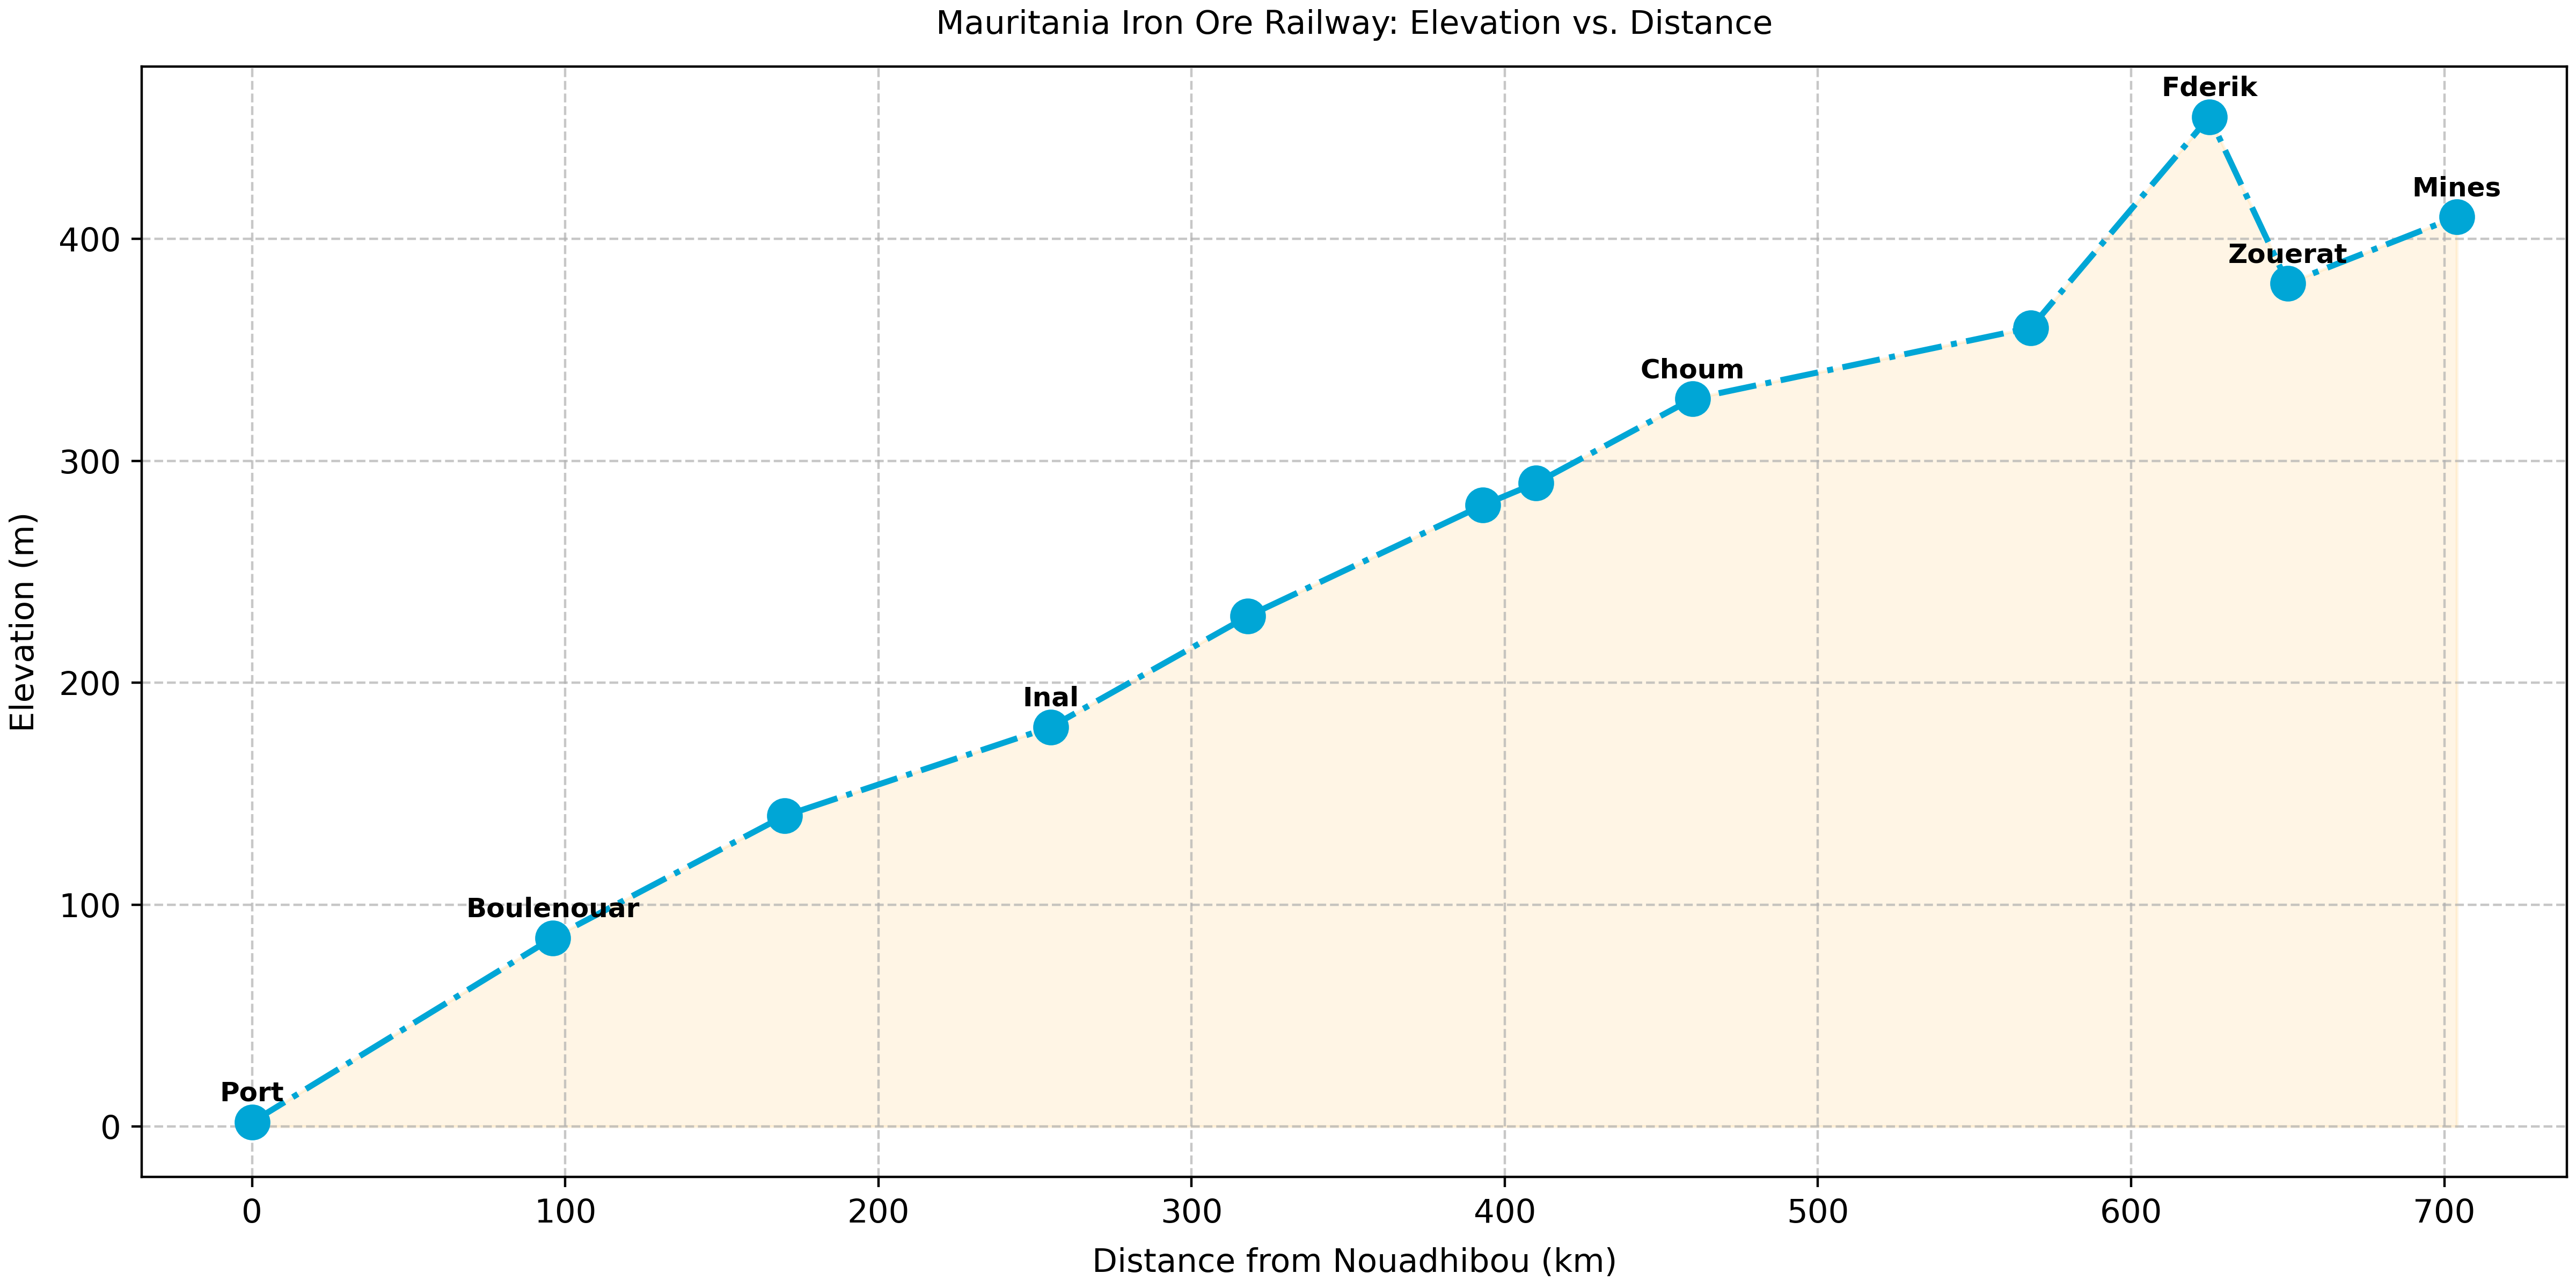
\includegraphics[width=\textwidth]{plots/track_profile.png}
    \caption{The height map of the track, extracted from google earth data of the elevation along the route~\cite{googleearth2026}.}
    \label{fig:track_profile}
\end{figure}
Along its journey the train passes through five larger villages, where the train is reported to stop for the loading of small goods and occasionally people~\cite{ASECNA2024}. These stops, together with the start and end stations at the mines and the sea, are also depicted in~\autoref{fig:track_profile}.

\section{Design of the Driving Cycle}

Given the limited quantitive information about the train itself and its velocity during the journey, the driving cycle itself became part of the design process. It had to be designed how fast the train accelerates, its speed on different sections of the track, and how long the train stops. This section explains how the track sections were modelled and the driving cycle designed, based on the height profile and stops in~\autoref{fig:track_profile}.
In order to reasonably limit the design freedom, the goal was set for the train to finish the enitre journey in under~\qty{20}{\hour} and ~\qty{15}{\hour} for the west- and eastbound case, respectively. To not endanger machanical stability of the track rails, the top speeds of \qty{45}{\km\per\hour} and \qty{65}{\km\per\hour} were also kept as a hard design requirement. These values are all in approximate agreement with the current train journey.

From there on, calculations for the required traction power $P_t$ of the train for different scenarios, such as zero-gradient top speed, different accelerations and the incline part for the loaded train, were performed using
\begin{equation}\label{eq:traction_power}
    P_t = V \left( Mgf_r \cos \alpha + Mg \sin \alpha + \frac{1}{2} \rho A_f C_D (V)^2 + M \delta \frac{dV}{dt} \right)
\end{equation}
in order to find the maximum value for $P_t$. The parameters used for these calculations are listed in~\autoref{tab:drive_cycle_parameters}. 
\begin{table}[ht]
    \centering
    \caption{Parameters used for the traction power calculations of the train.}
    \label{tab:drive_cycle_parameters}
    \begin{tblr}{
        colspec={l c c},
        row{1} = {font=\bfseries},
        hlines,
        vlines
    }
        Parameter & Value & Description\\
         $V$& max. \qty{65}{\km\per\hour} (unloaded), \qty{45}{\km\per\hour} (loaded) & maximum velocity of the train\\
        $M$ & \qty{5e6}{\kg} (unloaded), \qty{22e6}{\kg} (loaded) & mass of the train \\ 
        $g$ & \qty{9.81}{\meter\per\second\squared} & gravitational acceleration \\
        $f_r$ & \qty{0.0015}{} & rolling resistance coefficient\\
         $\alpha$& max. \qty{0.0036}{rad} (loaded), \qty{0.0015}{rad} (unloaded) & (maximum) incline angle\\
         $A_f$& \qty{12}{\meter\squared} & aerodynamic frontal train area\\
         $c_D$& \qty{1}{} & aerodynamic drag coefficient\\
         $\delta$& \qty{1.02}{} & mass factor due to inertia\\
    \end{tblr}
\end{table}
It has to be noted, that~\autoref{eq:traction_power} assumes zero wind speed, to simplify the areodynamic power loss estimations (in~\autoref{sec:Simulation} it is shown that aerodynamic forces are relatively small anyways). Further, the maximum incline angle is small enough for the approximation of $\cos \alpha \approx 1$ and $\sin \alpha \approx \alpha$ to be used in~\autoref{eq:traction_power}. The resulting values for $P_t$ were then compared to each other to identify the section that requires the most power and to evaluate, if it makes sense to reduce this power, e.g. by lowering the speed or acceleration, in order to avoid oversizing of the powertrain for one section.

For simplicity of the model, it was assumed that the train accelerates to a constant speed in between stops and only slows down to come to a halt at the next village. This leaves the question of the target speed in between sections and the acceleration profile open, to fully define the drive cycle.
\subsection{Steady state speed design}
% plot with power for steady state top speed on flat and on max. incline
In the most simple version of the driving cycle, the target speed would always be equal to the maximum possible top speed after~\autoref{tab:drive_cycle_parameters}. From a power perspective, the most demanding section in steady state ($\frac{dV}{dt}=0$) is the one with the maximum incline angle $\alpha_{max}$. Thus, steady state power calculations for the maximum incline on both the loaded and unloaded journey were done and depicted in~\autoref{fig:steady_state_power} for the respective top speeds.   
\begin{figure}[ht]
    \centering
    
\includegraphics[]{EV_Project - Mauretanian Train/plots/peak_power.pdf}
    \caption{Steady state traction power for zero and maximum gradient for both, the unloaded and loaded train journey.}
    \label{fig:steady_state_power}
\end{figure}
% explain how we changed max speed on loaded incline to get power ratings down
As expected it can be seen that the maximum traction power, is required on the incline part of the loaded journey. Since it exceeds \qty{13.6}{\MW} for a speed of \qty{45}{\km\per\hour} on that section, the target speed was limited to \qty{30}{\km\per\hour}. This archieves a compromise between journey time and the peak power that has to be provided. Since on all other sections, the incline is actually negative for the loaded train, the required steady state power will always be lower than the \qty{4}{\MW} in~\autoref{fig:steady_state_power} and the target speed was set to \qty{45}{\km\per\hour}. For the unloaded journey, the required traction power is lower, even on the steepest incline part, with the higher top speed. The target speed was therefore set to \qty{65}{\km\per\hour} for all sections.
\subsection{Train acceleration design}
The acceleration of the train after a stop had the greatest freedom of design. By looking at other heavy-duty trains of similar size and weight, it could be concluded, that a maximum acceleration of~\qty{0.1}{\meter\per\second\squared} is sufficient.
Since the traction power required to archieve a specific acceleration in~\autoref{eq:traction_power} increases with increasing speed, a constant acceleration is not a realistic model and would result in a spiking power for higher speeds. That is even more the case, since the resistive forces also increase with speed. To account for this, while still keeping a reasonably simple, quasi-static model, three different acceleration levels from stantstill up to the respective topspeed were chosen. The values for these acceleration levels were iteratively determined, by starting with educated guesses, that roughly keep $\frac{dV}{dt}\propto V^{-1}$, then computing the corresponding drive cycle for one acceleration period to top speed with a python skript, and finally calculating the traction power over time curve with the QSS vehicle model (see~\autoref{sec:Simulation}). The acceleration levels were changed until the resulting traction power did not significantly exceed the maximum steady state power at maximum incline, to again avoid oversizing. The final values for the train acceleration as well as their cut off speeds are listed in~\autoref{tab:acceleration_levels}.
% Acceleration Table

\begin{table}[ht]
    \centering
    \caption{Acceleration levels for the train starting from standstill and their corresponding cut off speeds, up until it is used.}
    \label{tab:acceleration_levels}
    \begin{tblr}{
        colspec={c c c c },
        column{1} = {font=\bfseries},
        hlines,
        vlines
    }
        $V_{cut,off}$ (loaded) in \si{\m\per\second} & 15 & 30 & -\\
        $V_{cut,off}$ (unloaded) in \si{\m\per\second} & 20 & 40 & -\\
        acceleration in \si{\m\per\second\squared}& 0.08 & 0.04 & 0.02\\
    \end{tblr}

\end{table}
It has to be noted, that these values were designed for the loaded train on the stop with the least negative gradient. Since there is a stop on the loaded journey directly before the steep incline, the train also has to accelerate on that part. To keep the power withing limits, a very slow acceleration of \qty{0.02}{\m\per\second\squared} was taken for the modelling of the loaded driving cycle after the first stop.

For the final values, one full acceleration period, as well as the corresponding traction power curve are shown in~\autoref{fig:examp_accel} after the stop in Inal.
\begin{figure}[ht]
    \centering
    
\includegraphics[width=0.9\textwidth]{EV_Project - Mauretanian Train/plots/example_acceleration_period.png}
    \caption{Example of one acceleration period to loaded top speed of~\qty{45}{\km\per\hour}.}
    \label{fig:examp_accel}
\end{figure}
It can be observed, that the peak power stays below \qty{10}{\MW}, due to the three acceleration levels. Note that an additional starting acceleration level, for speeds below \qty{5}{\km\per\hour} is also present. This was added later in the design process, to limit the output power of the electric motor at very low speeds, where induction machines operate with a low efficiency. With the acceleration levels set, the final driving cycles could be created and imported into QSS together with the track slope that was extrapolated from the height map in~\autoref{fig:track_profile}. They are shown in~\autoref{fig:driving_cycle} for the loaded and unloaded journey. 
\begin{figure}[ht]
    \centering
    
\includegraphics{EV_Project - Mauretanian Train/plots/drive_cycle.png}
    \caption{Final driving cycles for the loaded and unloaded journey.}
    \label{fig:driving_cycle}
\end{figure}
% explain iterative acceleration profile determination: set acceleration profiles --> get drive cycle --> evaluate max power in qss --> repeat
% explain 3 accell levels
% explain
\newpage
\section{Design of the Powertrain}
\newpage
\input{chapters/03_Simulation.tex}
\newpage
\input{chapters/04_Charging_Islands}

\newpage
\addcontentsline{toc}{section}{References}
\bibliographystyle{IEEEtran}~\nocite{*}
\bibliography{reference/ref}

\end{document}